\documentclass[dvipdfmx,fleqn]{beamer}
%\documentclass[dvipdfmx,fleqn,handout]{beamer}
\usepackage{amsmath,amssymb,amsthm}

\mode<presentation>
{
  \usetheme{default}
}

\title{\Large Fictitious Play}
\author{\large 山岸 敦}
\date{\small 2014/6/28}

\usefonttheme{professionalfonts}

\setbeamercovered{transparent=20}

\setbeamertemplate{navigation symbols}{} 
\setbeamertemplate{footline}[frame number] 



\begin{document}

\sffamily
\gtfamily


\begin{frame}
  \titlepage
  \thispagestyle{empty}
\end{frame}

\setcounter{framenumber}{0}




\begin{frame}
\frametitle{構成}
\begin{itemize}\setlength{\parskip}{0.5em}
\item
Fictitious Playとは?
\item
シミュレーション結果の解説
 \begin{itemize}\setlength{\parskip}{0.5em}
 \item
Matching Pennies Game
 \item
 Coordination Game
 \end{itemize}

\item
Pythonコードの解説
\end{itemize}
\end{frame}



\begin{frame}
\frametitle{Fictitious Playの解説}
\begin{itemize}\setlength{\parskip}{0.5em}
\item
Ficititious playでは、相手の前回の行動により、「相手がどの手をどんな確率で出してくるか」についての予想(信念)が変化する状況が想定されます。\pause

\item
さらにどの時点でも、プレイヤーは「その時点での自信の信念に照らして最適」な行動をするとします。このとき、各人の信念の動きはどうなるのでしょうか?\pause
\item
信念の推移を定式化すると、(導出は省略しますが) 

$x_0(t)$ は
\[
x_0(t+1)
= x_0(t) + \frac{1}{t+2} (a_1(t) - x_0(t))
\]
と再帰的に書くことができます。 



\end{itemize}
\end{frame}

\begin{frame}
\frametitle{Matching Pennies Gameの解説}
\begin{itemize}\setlength{\parskip}{0.5em}
\item
Matching Pennies Gameの利得行列は
\[\left( \begin{array}{cc}
(1,-1) & (-1,1) \\
(-1,1) & (1,-1) 
\end{array} \right)\]
です。ナッシュ均衡は両戦略に確率(0.5,0.5)ずつ付与する混合戦略のみであることがわかります。\pause

\item
お互いの信念が(0.5,0.5)に収斂するならば、ナッシュ均衡が実現する、と考えてよいでしょう\pause
\item
本当にそうなるか、シミュレーションした結果を示します。



\end{itemize}
\end{frame}


\begin{frame}
\frametitle{}
\begin{figure}
 \centering
 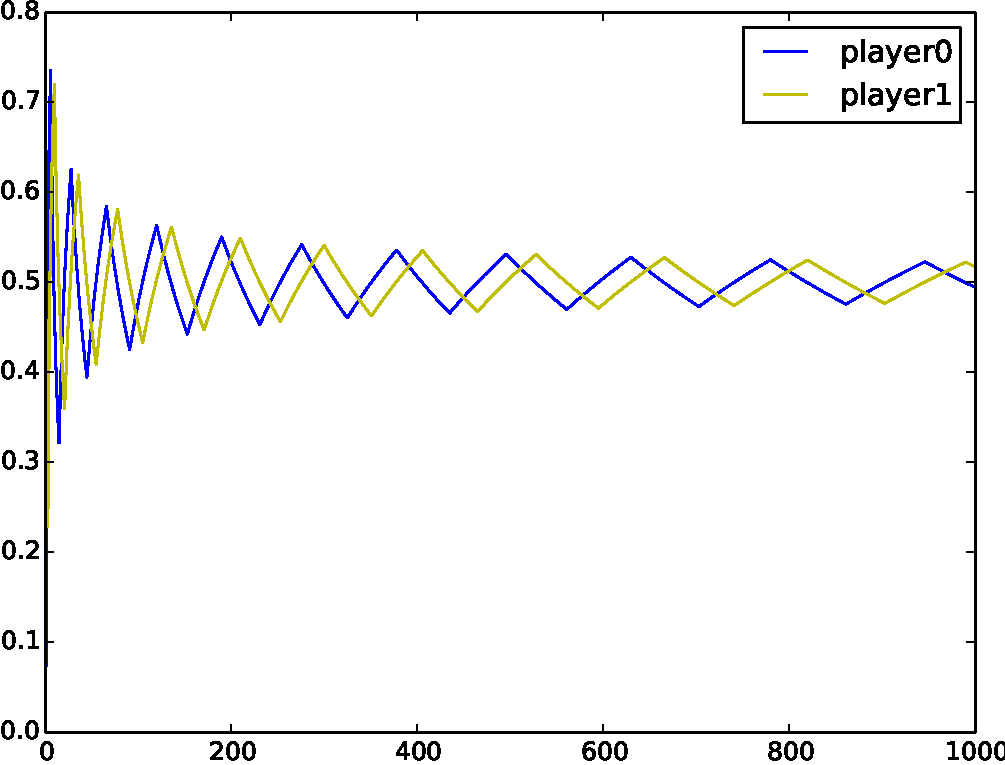
\includegraphics[scale=0.58, bb=-250 -200 250 200]{fictitious_graph1.0.pdf}
 \caption{Matching Pennies Game}
 \label{fig:matchingpennies_plot}
\end{figure}
\end{frame}

\begin{frame}
\frametitle{}
\begin{figure}
 \centering
 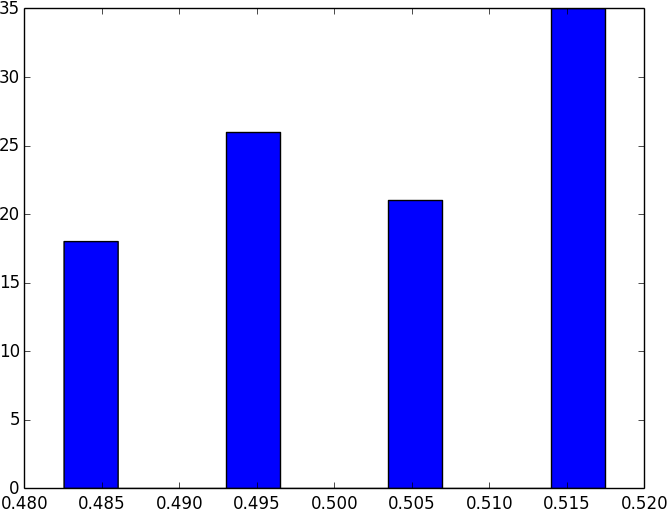
\includegraphics[scale=0.58, bb=-250 -200 250 200]{fictitious_histo1.0.png}
 \caption{Matching Pennies Game}
 \label{fig:matchingpennies_histo}
\end{figure}
\end{frame}

\begin{frame}
\frametitle{Coordination Gameの解説}
\begin{itemize}\setlength{\parskip}{0.5em}
\item
Coordination Gameの利得行列は
\[\left( \begin{array}{cc}
(4,4) & (0,3) \\
(3,0) & (2,2) 
\end{array} \right)\]
です。ナッシュ均衡は純粋戦略の組(0,0)、(1,1)および、2人とも確率(2/3,1/3)ずつ付与する混合戦略の3つです。\pause

\item
先程とちがって、ナッシュ均衡が複数あります。このケースではどのようなプレイがなされるのでしょうか\pause
\item
シミュレーションした結果を示します。



\end{itemize}
\end{frame}

\begin{frame}
\frametitle{}
\begin{figure}
 \centering
 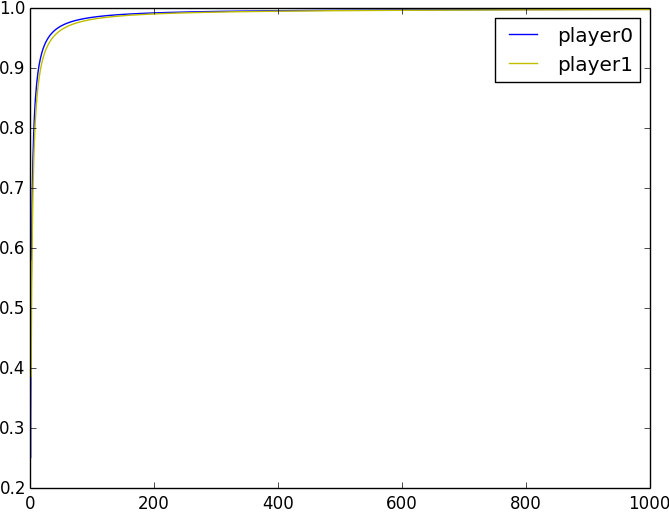
\includegraphics[scale=0.58, bb=-250 -200 250 200]{coordinationgame_graph1.png.png}
 \caption{Coordination Game}
 \label{fig:coordination_plot1}
\end{figure}
\end{frame}


\begin{frame}
\frametitle{}
\begin{figure}
 \centering
 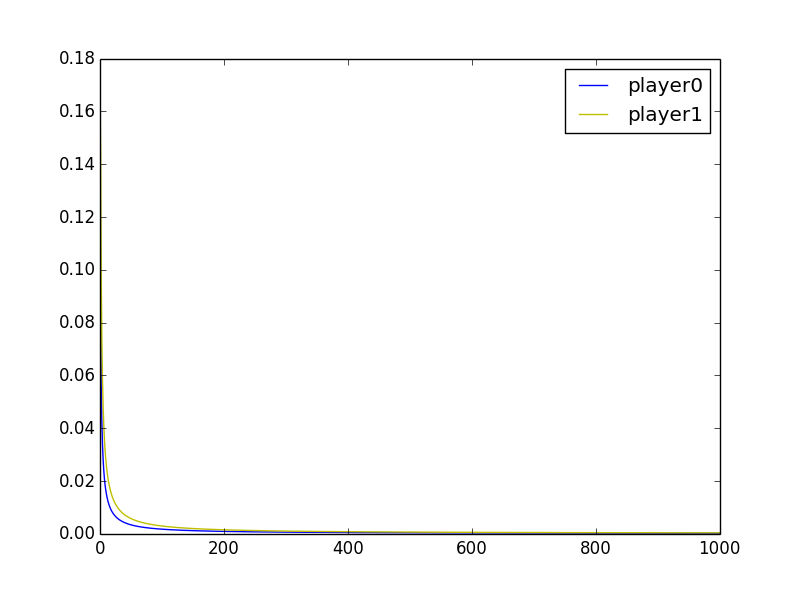
\includegraphics[scale=0.58, bb=100 200 400 300]{coordinationgame_graph2.png}
 \label{fig:coordination_plot2}
\end{figure}
\end{frame}

\begin{frame}
\frametitle{}
\begin{figure}
 \centering
 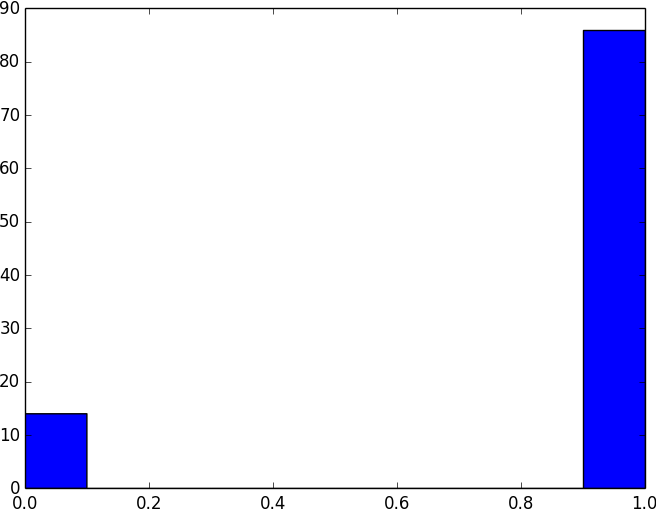
\includegraphics[scale=0.58, bb=-250 -200 250 200]{coordination_histo1.0.png}
 \caption{Coordination Game}
 \label{fig:coordination_histo}
\end{figure}
\end{frame}




\begin{frame}
\frametitle{補足:Coordination Game}
\begin{itemize}\setlength{\parskip}{0.5em}
\item
各プレイヤーは「相手が2/3より大きい確率で0をプレイするなら0を、それが2/3より小さければ1を」必ず選択します。よって、混合戦略均衡で、たまたまお互いに0ないし1を取ればそちらの均衡に移るとわかります。ヒストグラムを眺めると、混合戦略に収斂した回数はゼロです。 \pause
\item
「両者にとって、相手が均衡(純)戦略を取る確率が$p$以上の時、自分もその均衡(純)戦略を取るのが最適である」ならば、その戦略の組み合わせは$p$-ドミナントと呼ばれます。\pause
\item
(0,0)は2/3ドミナント、(1,1)は1/3ドミナントです。一般に「相手が均衡(純)戦略を取る確率がより低くても最適」という意味で$p$が小さいほうが安全で起こりやすい均衡と予想されます。\pause
\item
ヒストグラムを眺めると、(0,0)均衡と比して(1,1)均衡がプレイされる頻度が圧倒的に大きいですが、これによりある(それなりにもっともらしい)信念形成過程を仮定した下で$p$ドミナントの性質が確認できた、と言えると思います。

\end{itemize}
\end{frame}




\begin{frame}[containsverbatim]% verbatim 環境を使えるように
\frametitle{Matching Pennies Game:コードの解説}
\begin{itemize}\setlength{\parskip}{0.5em}
\item
まずは必要な物をimportし、利得をnparrayで設定します。これを用いると後々期待利得の計算などがラクになります。
\begin{verbatim}
from __future__ import division
import matplotlib.pyplot as plt
import random 
import numpy as np



#defining variables and functions that are useful

payoff_0 = np.array([[1,-1],[-1,1]])
payoff_1 = np.array([[-1,1],[1,-1]])


\end{verbatim}

\
\end{itemize}
\end{frame}


\begin{frame}[containsverbatim]% verbatim 環境を使えるように
\frametitle{Matching Pennies Game:コードの解説}
\begin{itemize}\setlength{\parskip}{0.5em}
\item
次に、必要な関数を定義していきます。ついでに、初期信念もここで設定しています。
\begin{verbatim}
def set_intbelief():
	int_belief = random.uniform(0,1)
	return  np.array([1-int_belief,int_belief])
	 # belief about the opponent's actions

belief0 = set_intbelief()
belief1 = set_intbelief()

def expected_value(payoff,beliefs):
	return np.dot(payoff,beliefs)
	# returns expected values of each action as a vector


\end{verbatim}
\end{itemize}
\end{frame}


\begin{frame}[containsverbatim]% verbatim 環境を使えるように
\frametitle{Matching Pennies Game:コードの解説}
\begin{itemize}\setlength{\parskip}{0.5em}
\item
引き続き、必要な関数を定義していきます。あと、後にグラフを書くのに使うリストTrajectoryを設定しています。
\begin{verbatim}
def take_action(x)
: # this takes a vector as an argument

	if x[0] > x[1]:
		return 0
	elif x[0] < x[1]:
		return 1
	else:
		return random.randint(0,1)

# lists used later to draw the graph
trajectory0 = [belief0[1]]
trajectory1 = [belief1[1]]

\end{verbatim}
\end{itemize}
\end{frame}

\begin{frame}[containsverbatim]% verbatim 環境を使えるように
\frametitle{Matching Pennies Game:コードの解説}
\begin{itemize}\setlength{\parskip}{0.5em}
\item
for文で、ゲームをプレイ。信念の軌跡はTrajectoryに保存
\begin{verbatim}
for i in range(1000):

	ev0 = expected_value(payoff_0,belief0)
	ev1 = expected_value(payoff_1,belief1)

	action0 = take_action(ev0)
	action1 = take_action(ev1)

	# updating beliefs
	m = belief0[1] + (action1 - belief0[1])/(i + 2)
	n = belief1[1] + (action0 - belief1[1])/(i + 2)
	belief0 = np.array([1-m,m])
	belief1 = np.array([1-n,n])

	trajectory0.append(belief0[1])
	trajectory1.append(belief1[1])
\end{verbatim}
\end{itemize}
\end{frame}

\begin{frame}[containsverbatim]% verbatim 環境を使えるように
\frametitle{Matching Pennies Game:コードの解説}
\begin{itemize}\setlength{\parskip}{0.5em}
\item
描画します。\verb!#!を取ると画像が保存できます。
\begin{verbatim}
plt.plot(trajectory0, 'b-', label='player0')  
plt.plot(trajectory1, 'y-', label='player1')  
plt.legend()
#plt.savefig
#("fictitious_graph1.0.png"
,bbox_inches="tight",pad_inches=0)

plt.show()

\end{verbatim}
\item
ヒストグラムもほぼ同様のプログラムです。このプログラムを、さらにfor文でメタ的に包み込む形になります。

\end{itemize}
\end{frame}

\begin{frame}
\frametitle{まとめ}
\begin{itemize}\setlength{\parskip}{0.5em}
\item
二種類のゲームをプレイさせて、どんな戦略の組が均衡になるか調べることができます。今回僕が試したゲーム以外では、永遠に均衡にたどり着かないケースもありそうです。\pause

\item
ヒストグラムを描くときにforループを二重にするという原始的手法を用いましたが、処理回数が指数的に増加しているのでもっさりしています。
どう改善できるのでしょうか…\pause
\item
2人2戦略ゲームについては、それなりに一般性の高いコードが書けたと思います。
しかし、ここからn人、n戦略へと拡張するならば複雑性が増し、classを定義して整理していく必要が生まれそうです。\pause
\item
今回は、classについては逆に複雑になる+恩恵が薄い気がしたので避けましたが、もう少し複雑なバージョンをclassで書いて将来的には使いこなせるように練習したい。\pause
\end{itemize}
\end{frame}




\end{document}